

\begin{center}
\thispagestyle{empty}
%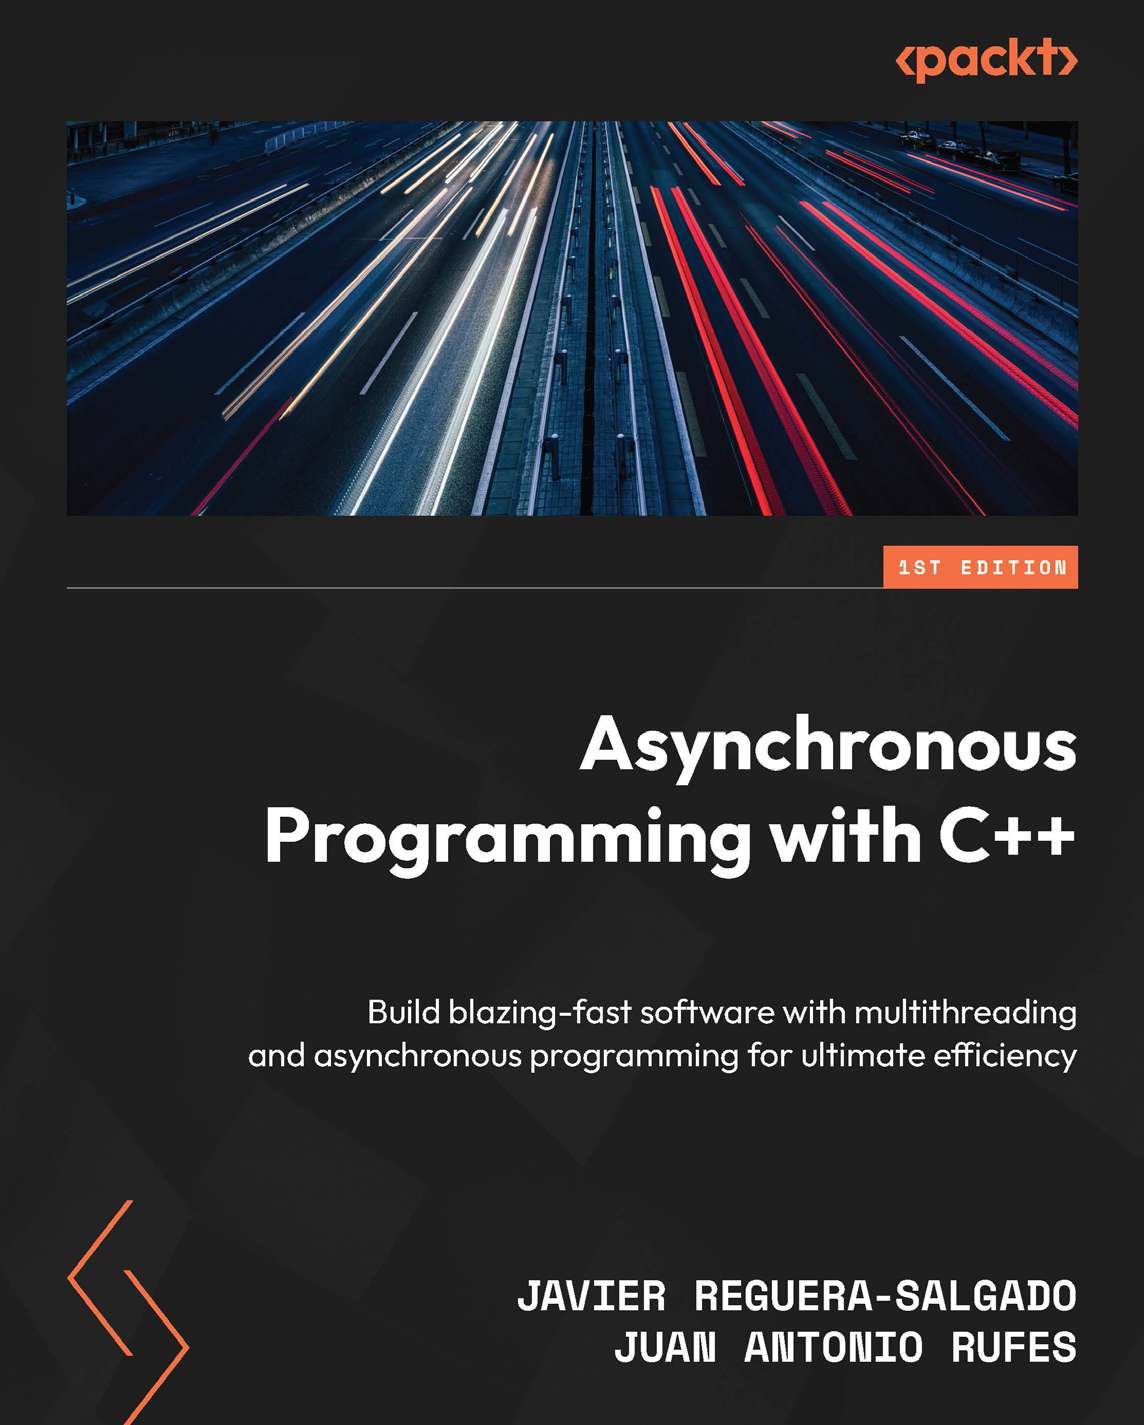
\includegraphics[width=\textwidth,height=\textheight,keepaspectratio]{cover.png}
\begin{tikzpicture}[remember picture, overlay, inner sep=0pt]
\node at (current page.center)
{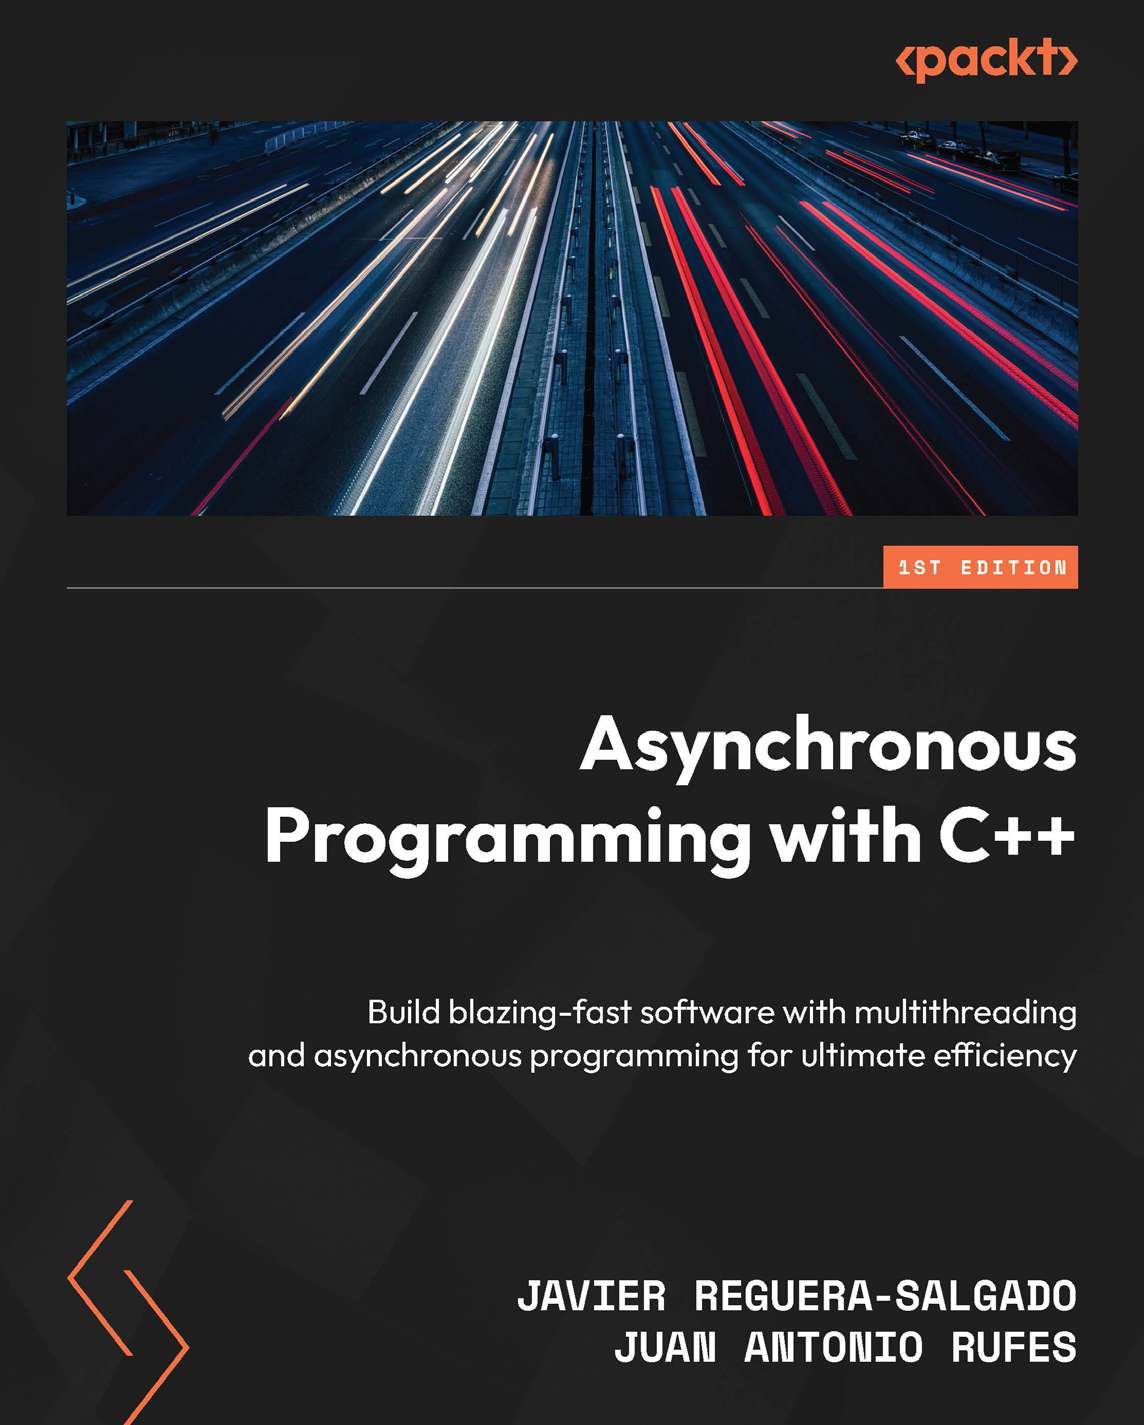
\includegraphics[width=\paperwidth, keepaspectratio=false]{cover.png}};
\end{tikzpicture}
\newpage
\thispagestyle{empty}
\huge
\textbf{Asynchronous Programming with C++}
\\[9pt]
{\Large 通过多线程和异步编程打造高速运行的软件}
\\[9pt]
\normalsize
作者: Javier Reguera-Salgado / Juan Antonio Rufes
\\[8pt]
\normalsize
译者:\href{https://github.com/xiaoweiChen/Asynchronous-Programming-with-Cpp}{陈晓伟}
\\[8pt]
\end{center}

\newpage

\begin{comment}
\end{comment}

\myChapterNoContents{致谢}{}{content/acknowledgments.tex}
\newpage

\myChapterNoContents{关于作者}{}{content/contributors.tex}
\newpage

\myChapterNoContents{关于评审}{}{content/reviewers.tex}
\newpage


\pagestyle{empty}
\tableofcontents
\newpage

\setsecnumdepth{section}

\myChapter{前言}{}{content/preface.tex}
\newpage

\myPartGray{第一部分}{并行编程和流程管理}{content/part1/part.tex}
\newpage


\myChapter{第1章}{并行编程范式}{content/part1/chapter1/0.tex}
\mySubsection{1.1.}{技术要求}{content/part1/chapter1/1.tex}
\mySubsection{1.2.}{分类、技术和模型}{content/part1/chapter1/2.tex}
\mySubsection{1.3.}{并行编程范式}{content/part1/chapter1/3.tex}
\mySubsection{1.4.}{并行性指标}{content/part1/chapter1/4.tex}
\mySubsection{1.5.}{总结}{content/part1/chapter1/5.tex}
\mySubsection{1.6.}{扩展阅读}{content/part1/chapter1/6.tex}
\newpage

\myChapter{第2章}{进程、线程和服务}{content/part1/chapter2/0.tex}
\mySubsection{2.1.}{Linux 中的进程}{content/part1/chapter2/1.tex}
\mySubsection{2.2.}{Linux 中的服务和守护进程}{content/part1/chapter2/2.tex}
\mySubsection{2.3.}{线程}{content/part1/chapter2/3.tex}
\mySubsection{2.4.}{同步原语}{content/part1/chapter2/4.tex}
\mySubsection{2.5.}{使用多线程时的常见问题}{content/part1/chapter2/5.tex}
\mySubsection{2.6.}{有效线程管理的策略}{content/part1/chapter2/6.tex}
\mySubsection{2.7.}{总结}{content/part1/chapter2/7.tex}
\mySubsection{2.8.}{扩展阅读}{content/part1/chapter2/8.tex}
\newpage

\myPartGray{第二部分}{高级线程管理和同步技术}{content/part2/part.tex}
\newpage

\myChapter{第3章}{如何在 C++ 中创建和管理线程}{content/part2/chapter3/0.tex}
\mySubsection{3.1.}{技术要求}{content/part2/chapter3/1.tex}
\mySubsection{3.2.}{线程库 – 简介}{content/part2/chapter3/2.tex}
\mySubsection{3.3.}{线程操作}{content/part2/chapter3/3.tex}
\mySubsection{3.4.}{线程本地存储}{content/part2/chapter3/4.tex}
\mySubsection{3.5.}{实现计时器}{content/part2/chapter3/5.tex}
\mySubsection{3.6.}{总结}{content/part2/chapter3/6.tex}
\mySubsection{3.7.}{扩展阅读}{content/part2/chapter3/7.tex}
\newpage

\myChapter{第4章}{使用锁进行线程同步}{content/part2/chapter4/0.tex}
\mySubsection{4.1.}{技术要求}{content/part2/chapter4/1.tex}
\mySubsection{4.2.}{了解条件竞争}{content/part2/chapter4/2.tex}
\mySubsection{4.3.}{为什么需要互斥?}{content/part2/chapter4/3.tex}
\mySubsection{4.4.}{管理通用锁}{content/part2/chapter4/4.tex}
\mySubsection{4.5.}{条件变量}{content/part2/chapter4/5.tex}
\mySubsection{4.6.}{实现多线程安全队列}{content/part2/chapter4/6.tex}
\mySubsection{4.7.}{信号量}{content/part2/chapter4/7.tex}
\mySubsection{4.8.}{栅栏和门闩}{content/part2/chapter4/8.tex}
\mySubsection{4.9.}{仅执行一次任务}{content/part2/chapter4/9.tex}
\mySubsection{4.10.}{总结}{content/part2/chapter4/10.tex}
\mySubsection{4.11.}{扩展阅读}{content/part2/chapter4/11.tex}
\newpage

\myChapter{第5章}{原子操作}{content/part2/chapter5/0.tex}
\mySubsection{5.1.}{技术要求}{content/part2/chapter5/1.tex}
\mySubsection{5.2.}{原子操作简介}{content/part2/chapter5/2.tex}
\mySubsection{5.3.}{非阻塞数据结构}{content/part2/chapter5/3.tex}
\mySubsection{5.4.}{C++ 内存模型}{content/part2/chapter5/4.tex}
\mySubsection{5.5.}{C++ 标准库原子类型和操作}{content/part2/chapter5/5.tex}
\mySubsection{5.6.}{SPSC 无锁队列}{content/part2/chapter5/6.tex}
\mySubsection{5.7.}{总结}{content/part2/chapter5/7.tex}
\mySubsection{5.8.}{扩展阅读}{content/part2/chapter5/8.tex}
\newpage

\myPartGray{第三部分}{使用 Promise、 Future和协程}{content/part3/part.tex}
\newpage

\myChapter{第6章}{Promise和Future}{content/part3/chapter6/0.tex}
\mySubsection{6.1.}{技术要求}{content/part3/chapter6/1.tex}
\mySubsection{6.2.}{探索Promise和Future}{content/part3/chapter6/2.tex}
\mySubsection{6.3.}{Promise 和 Future 的优点和缺点}{content/part3/chapter6/3.tex}
\mySubsection{6.4.}{现实场景和解决方案的示例}{content/part3/chapter6/4.tex}
\mySubsection{6.5.}{总结}{content/part3/chapter6/5.tex}
\mySubsection{6.6.}{扩展阅读}{content/part3/chapter6/6.tex}
\newpage

\myChapter{第7章}{异步函数}{content/part3/chapter7/0.tex}
\mySubsection{7.1.}{技术要求}{content/part3/chapter7/1.tex}
\mySubsection{7.2.}{什么是std::async?}{content/part3/chapter7/2.tex}
\mySubsection{7.3.}{启动策略}{content/part3/chapter7/3.tex}
\mySubsection{7.4.}{处理异常}{content/part3/chapter7/4.tex}
\mySubsection{7.5.}{异步 Future 和性能}{content/part3/chapter7/5.tex}
\mySubsection{7.6.}{限制线程数}{content/part3/chapter7/6.tex}
\mySubsection{7.7.}{何时不应使用 std::async}{content/part3/chapter7/7.tex}
\mySubsection{7.8.}{实例}{content/part3/chapter7/8.tex}
\mySubsection{7.9.}{总结}{content/part3/chapter7/9.tex}
\mySubsection{7.10.}{扩展阅读}{content/part3/chapter7/10.tex}
\newpage

\myChapter{第8章}{使用协程}{content/part3/chapter8/0.tex}
\mySubsection{8.1.}{技术要求}{content/part3/chapter8/1.tex}
\mySubsection{8.2.}{协程}{content/part3/chapter8/2.tex}
\mySubsection{8.3.}{C++ 协程}{content/part3/chapter8/3.tex}
\mySubsection{8.4.}{实现协程}{content/part3/chapter8/4.tex}
\mySubsection{8.5.}{协程生成器}{content/part3/chapter8/5.tex}
\mySubsection{8.6.}{简单的协程字符串解析器}{content/part3/chapter8/6.tex}
\mySubsection{8.7.}{协程和异常}{content/part3/chapter8/7.tex}
\mySubsection{8.8.}{总结}{content/part3/chapter8/8.tex}
\mySubsection{8.9.}{扩展阅读}{content/part3/chapter8/9.tex}
\newpage

\myPartGray{第四部分}{使用Boost库进行高级异步编程}{content/part4/part.tex}
\newpage

\myChapter{第9章}{使用 Boost.Asio 进行异步编程}{content/part4/chapter9/0.tex}
\mySubsection{9.1.}{技术要求}{content/part4/chapter9/1.tex}
\mySubsection{9.2.}{什么是 Boost.Asio?}{content/part4/chapter9/2.tex}
\mySubsection{9.3.}{与操作系统交互}{content/part4/chapter9/3.tex}
\mySubsection{9.4.}{Reactor 和 Proactor 设计模式}{content/part4/chapter9/4.tex}
\mySubsection{9.5.}{使用 Boost.Asio 进行线程处理}{content/part4/chapter9/5.tex}
\mySubsection{9.6.}{管理对象的生命周期}{content/part4/chapter9/6.tex}
\mySubsection{9.7.}{使用缓冲区传输数据}{content/part4/chapter9/7.tex}
\mySubsection{9.8.}{信号处理}{content/part4/chapter9/8.tex}
\mySubsection{9.9.}{取消操作}{content/part4/chapter9/9.tex}
\mySubsection{9.10.}{使用 strands 序列化工作负载}{content/part4/chapter9/10.tex}
\mySubsection{9.11.}{协程}{content/part4/chapter9/11.tex}
\mySubsection{9.12.}{总结}{content/part4/chapter9/12.tex}
\mySubsection{9.13.}{扩展阅读}{content/part4/chapter9/13.tex}
\newpage

\myChapter{第10章}{使用 Boost.Cobalt 实现协程}{content/part4/chapter10/0.tex}
\mySubsection{10.1.}{技术要求}{content/part4/chapter10/1.tex}
\mySubsection{10.2.}{Boost.Cobalt 库简介}{content/part4/chapter10/2.tex}
\mySubsection{10.3.}{Boost.Cobalt生成器}{content/part4/chapter10/3.tex}
\mySubsection{10.4.}{Boost.Cobalt 任务和promise}{content/part4/chapter10/4.tex}
\mySubsection{10.5.}{Boost.Cobalt 通道}{content/part4/chapter10/5.tex}
\mySubsection{10.6.}{Boost.Cobalt 同步函数}{content/part4/chapter10/6.tex}
\mySubsection{10.7.}{总结}{content/part4/chapter10/7.tex}
\mySubsection{10.8.}{扩展阅读}{content/part4/chapter10/8.tex}
\newpage

\myPartGray{第五部分}{异步编程的调试、测试和性能优化}{content/part5/part.tex}
\newpage

\myChapter{第11章}{记录和调试异步软件}{content/part5/chapter11/0.tex}
\mySubsection{11.1.}{技术要求}{content/part5/chapter11/1.tex}
\mySubsection{11.2.}{如何使用日志记录来发现错误}{content/part5/chapter11/2.tex}
\mySubsection{11.3.}{如何调试异步软件}{content/part5/chapter11/3.tex}
\mySubsection{11.4.}{总结}{content/part5/chapter11/4.tex}
\mySubsection{11.5.}{扩展阅读}{content/part5/chapter11/5.tex}
\newpage

\myChapter{第12章}{消杀和测试异步软件}{content/part5/chapter12/0.tex}
\mySubsection{12.1.}{技术要求}{content/part5/chapter12/1.tex}
\mySubsection{12.2.}{消杀代码以分析软件并查找潜在问题}{content/part5/chapter12/2.tex}
\mySubsection{12.3.}{测试异步代码}{content/part5/chapter12/3.tex}
\mySubsection{12.4.}{总结}{content/part5/chapter12/4.tex}
\mySubsection{12.5.}{扩展阅读}{content/part5/chapter12/5.tex}
\newpage

\myChapter{第13章}{提高异步软件性能}{content/part5/chapter13/0.tex}
\mySubsection{13.1.}{技术要求}{content/part5/chapter13/1.tex}
\mySubsection{13.2.}{性能测量工具}{content/part5/chapter13/2.tex}
\mySubsection{13.3.}{伪共享}{content/part5/chapter13/3.tex}
\mySubsection{13.4.}{CPU缓存}{content/part5/chapter13/4.tex}
\mySubsection{13.5.}{SPSC无锁队列}{content/part5/chapter13/5.tex}
\mySubsection{13.6.}{总结}{content/part5/chapter13/6.tex}
\mySubsection{13.7.}{扩展阅读}{content/part5/chapter13/7.tex}
\newpage

\begin{comment}
\end{comment}
